% !TEX root = ../main.tex
\documentclass[../main.tex]{subfiles}

\begin{document}

Die Abbildung~\ref{fig:Organigramm} zeigt die Organisation der Projektgruppe
10. Das Team ist agil organisiert und nach Disziplinen strukturiert. Die
Verantwortung für Organisation, Werkstatt und Budget ist zusätzlich auf
einzelne Positionen verteilt.

\begin{figure}[h!]
    \centering
    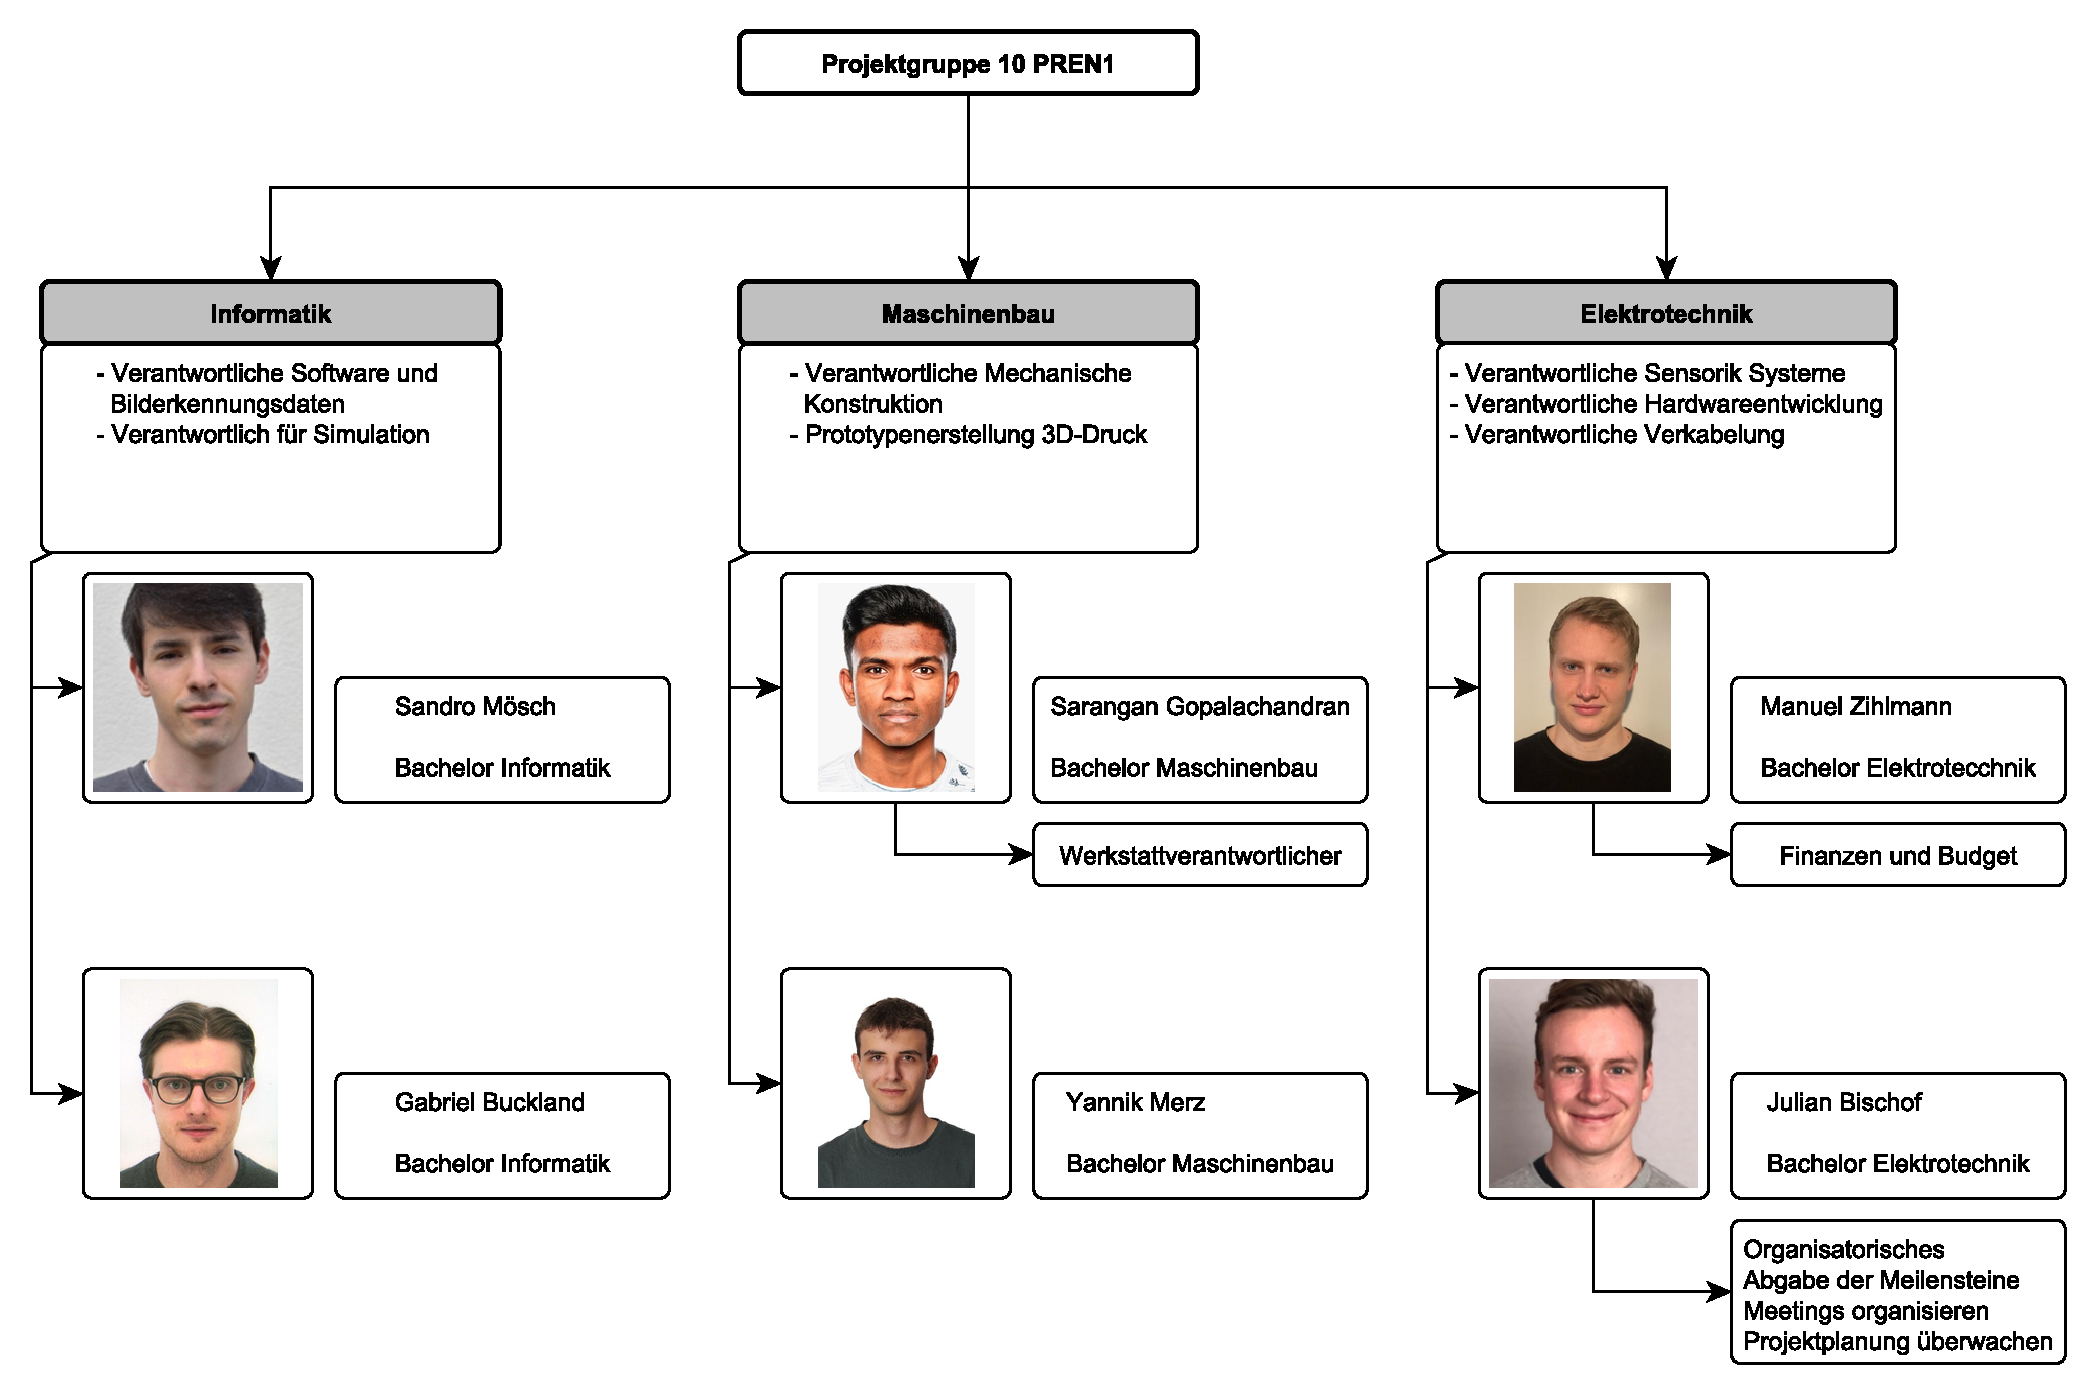
\includegraphics[page=1, width=1\textwidth]{../resources/Organigramm.pdf}
    \caption{Organigramm}\label{fig:Organigramm}
\end{figure}

\end{document}

